% !TeX root = ../main.tex

%TODO general chapter structure: short summar of following chapters, then "the following chapter explaines the process/architecture/usw in detail"

%TODO Bezüge zu Requirements!

\chapter{Implementation}\label{chapter:implementation}
The purpose of the tool is the continuous detection of copied code in a changing codebase.
The work of Koschke et al. makes clear that a index based approach seems appropriate for continuous detection:
\glqq If the [copy-paste detection] analysis is to be conducted multiple times, creating an index pays off\grqq \cite{koschke2014large}.

The index is based on the work of Hummel et al. \cite{hummel2010index}, where normalized sequences of statements of the code, which are called chunks, are hashed.
Other chunks of code can then be looked up by calculating the hash of those chunks the same way.
By comparing the resulting hashes with hashes in the index, locations of similar code can be found.

The tool is a client server architecture where the server stores a mapping of hash to location of the corresponding chunk.
It provides an interface to search for hashes.
The store for hashes is a key-value store where the key is the hash of a chunk of code.
The value contains information about the source of the chunk e.g. the url of the file or start and end positions within the file.

This chapter describes the architecture of the tool and technical details.
In the following, a target system is the codebase which should be scanned for copied code.
Reference systems are codebases which are indexed in the key-value store.

\section{System Overview}
\begin{figure}[h]
	\includegraphics{figures/architecture_overview.pdf}
	\caption{Tool Architecture Overview}\label{fig:tool_architecture}
\end{figure}
\autoref{fig:tool_architecture} shows an overview of the tool's architecture.
The server has a pool containing repositories of open source software available on the Internet.
The index is a key-value store where the key is the hash of a chunk.
The Indexer on the server regularly updates the repositories and re-indexes changes as described in \ref{section:implementation/creating_index}.
In that process, it also calculates the hash filter which can be downloaded by clients.

The client has a codebase which is watched by a scanner.
The scanner normalizes, groups statements and hashes those groups the same way the server does.
It then uses the resulting hash to search for copy-pasted code.
For that, the client sends the hash to the server, which looks up the value stored in the index using the hash as the key.
If a match could be found for the hash, the server responds with the origin of the corresponding chunk.
The client can use a hash filter as described in \autoref{section:implementation/creating_index/hash_filter} to reduce the amount of requests to the server and speed up the scanning process.
The hash filter can also be used as an offline solution by the client for finding sections of code in its codebase, where there is a high probability of copied code.

\section{Creating the Index}\label{section:implementation/creating_index}
This section describes the process which is done to create the index.
First, the code which should be indexed is normalized file-by-file.
For each file, the code is parsed and split into tokens.
A token represents a small part of the code such as a symbol, keyword, identifier, literal or comment.
The tokens then are normalized as described below.
Now the tokens are aggregated into statements.
The tool then passes over the resulting list of statements using a sliding window to group together a chunk of code, which consists of several consecutive statements.
The amount of statements in a chunk influences the precision of a match, since longer chunks also require longer matches.

The resulting chunks could be used to find similar code segments.
Hashing the chunks with a hash function reduces the space needed to store the information.
As a hash function, MD5 is used, since it offers both, speed and high collision resistance.
\autoref{fig:normalization} shows the complete processing of an input file.

A relational database may reduce the size of the store, because redundancy can be removed.
However, tests showed that even with bulk inserts, the creation of the database is more than 50 times slower than using a key-value store.
In this work RocksDB was used as a key-value store implementation, since it has proven to be very fast and space efficient.

\begin{figure}[h]
	\centering
	\begin{minipage}{1.2\linewidth}
		\begin{minipage}{0.35\linewidth}
			\scriptsize
			\lstinputlisting[language=C++]{data/buffer.c}
		\end{minipage}
		\begin{minipage}{0.23\linewidth}
			\scriptsize
			\begin{lstlisting}
			AVBufferRef * create uint8_t * data , ... !\tikzmark{bgnFir}!
			AVBufferRef * ref = NULL !\tikzmark{bgnSec}!
			AVBuffer * buf = NULL !\tikzmark{bgnThi}!
			buf = av_mallocz sizeof * buf
			if ! buf
			return NULL !\tikzmark{trmFir}!
			buf -> data = data !\tikzmark{trmSec}!
			buf -> size = size !\tikzmark{trmThi}!
			buf -> opaque = opaque
			atomic_init & buf -> refcount , 1
			...
			\end{lstlisting}
			
			%			\begin{tikzpicture}[overlay, remember picture]
			%			\drawBrace[.6em]{bgnFir}{trmFi}{Example xshifted.};
			%			\drawBrace{bgnSec}{trmSec}{Example annotation.};
			%			\drawBrace{bgnThi}{trmThi}{Another example.};
			%			\end{tikzpicture}
			
		\end{minipage}
	\end{minipage}
	\caption{Normalization Process}\label{fig:normalization}
\end{figure}

\subsection{Normalization}\label{section:implementation/creating_index/normalization}
The normalization step removes irrelevant information and by that, concentrates on the essential features of the code.
The parsing of code into tokens already does the first part of normalization by removing formatting.
After that, irrelevant tokens like access modifiers, import or include statements, comments or symbols like brackets or semicolons are removed.
The tokens which are left contain the main portion of information relevant for comparison of two sequences of code.
Since the tool should uncover mainly directly copied code, no further normalization is done.
In early tests, additionally normalizing identifiers like variable names showed many false positives for variable initializations e.g. in the beginning of methods.

\subsection{History Analysis}\label{section:implementation/creating_index/history_analysis}
As mentioned in section \ref{section:requirements/detecting_old_version}, it is important to also index old versions of the reference system.
The server regularly pulls changes form the open source repositories on the Internet.

To keep the index up to date and still keep information about older versions of the file, changed files are re-indexed.
For that, the server normalizes the new version of the file the same way as described before, groups it into chunks and hashes those chunks.
The resulting hashes are then inserted into the key value store.
If a hash already exists and links to a file with the same location, the old link is replaced with the new one.
This ensures, that a hash always points to the latest version of a file.
When files are deleted, nothing is changed in the key value store.

Instead of rescanning the whole file, only the chunks which have changed could be scanned.
However, the locations of hashes for chunks which did not change also have to be updated  in order to keep the latest version of a file in the index.

Changes to the repository can be seen in different granularity.
A fine granularity would be commit based.
On the one hand, this would ensure that the index contains the files' content at any given point in time.
On the other hand, the amount of changed files is huge with that and indexing large projects may take quite long.
First tests with a commit-based approach on the Linux kernel's master branch showed that a complete indexing would take several days to finish.
Note here that the Linux kernel code is a special case, since its master branch has more than 600000 commits on it.
Nonetheless, this test showed that commit based may be to slow for productive use.
Therefore, a tag based approach is used:
For each tag found in the reference system's repository, a re-index is triggered.
All changed files since the last tag are re-indexed again and the key-value store is updated as described before.

\subsection{Hash Filter}\label{section:implementation/creating_index/hash_filter}
It is expected, that most of the calculated hashes of a target system can not be found in the index.
Instead of having to send a request for every hash to the server, a better option would be a local copy of the index for faster lookup.
However, since the index may contain key-value pairs for billions lines of code, it is huge.
Distribution of the index to clients is a challenge, especially since the index has to be updated regularly.

With a table of all hashes contained in the index, the client would be able to lookup whether a hash is in the index and only has to send a request to the server in this rare case.
This could significantly speed up the analysis, since only hashes which actually are in the index would be looked up.
On the server-side this also reduces the load.

The size of the hash table is the amount of hashes times 128 bits which is the length of a MD5 hash.
Hashing with MD5 reduces the entropy of a chunk to about 128 bit of a ideal hash function.
Since lossless compression is expected not to reduce the size of the hashtable by much, lossy compression could be used.
One great way of reducing size of hash table with low false-positive probability is a BloomFilter.

To store a value, a BloomFilter uses multiple hash functions to hash a value. %TODO quelle?
It uses the resulting hash values as indexes to set bits of a bit array to 1.
To find out whether a value is stored in the BloomFilter, the value is hashed with the same hash functions as for storing a value.
Again, hash values are used as indexes.
If all values inside the bit array defined by the indexes are set to 1, the value is stored in the BloomFilter with a high probability.
If one or more of the bits are not set, the value is guaranteed not in the filter.
For the tool developed in this work, the values inserted into the BloomFilter are the hashes of the chunks.

The space $m$ in bits required to store $n$ values with the optimal number of hash functions can be estimated by $m = -\frac{n\cdot \ln(p)}{(\ln2)^{2}}$ with $p$ being the probability for a false positive.
For one billion hashes and a probability of 0.01\%, which roughly means one false positive for every 10000 lines of code, about 19170116755 bits or 2,4 GB are needed.
A simple hash table would need at least 128 billion bits or 16 GB for the same amount of data.

The advantage here is the small size of the filter.
However, the compression is lossy, because there is a certain probability for false positives.
The probability is depending on the size of the bit array, the number of inserted values and the number of used hash functions, but when kept at an optimum, grows almost linearly with the number of insertions.
Since it is not possible to remove values from the filter, it has to be recalculated every time the index changes.

It is also possible to only use the filter to find potential copied code.
This however, does not allow the client to find the origin for a potential match.
	
\section{Searching Copied Code}\label{section:implementation/searching_copied_code}
% TODO calculate probability of final false positive

\section{Future Work / Extensibility}\label{section:implementation/extensibility}
%TODO Extension points for future development? Web-Interface for code-add-request, Suggestions for linking libraries (gradle, ...)